%************************************************
\chapter{The Solvent Extraction Technique}\label{solventExtraction}
%************************************************
\begin{flushright}
February 19, 2013
\end{flushright}
\section{Aim}
To separate a given mixture of 2 colourless compounds, using the Solvent Extraction Technique, viz. Naphthol and Aniline.

\section {Chemicals Required}
	\begin{enumerate}
		\item Silica
		\item Iodine
		\item Ethyl Acetate
		\item Benzene
		\item Naphthol (given compound, refer to \autoref{e5_compound2})
		\item Aniline (given compound, refer to \autoref{e5_compound1})
		\item $NaHCO_3$ saturated solution
		\item $HCl$ ~ 1N
	\end{enumerate}

	\begin{figure}[bth]
		\begin{center}
			
\includegraphics[width=0.2\linewidth]{gfx/e5_compound1}
		\end{center}
	\caption[Aniline]{\label{e5_compound1}}
	\end{figure}

	\begin{figure}[bth]
		\begin{center}
			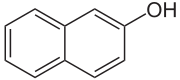
\includegraphics[width=0.4\linewidth]{gfx/e5_compound2}
		\end{center}
	\caption[2-Naphthol]{\label{e5_compound2}}
	\end{figure}

\section{Theory}
	The theory of this experiment is particularly elegant, as it's simple yet very powerful. Say if there are two compounds in a mixture, such that both have very close $R_f$ values and both are soluble in an organic solvent. The methods we've learnt so far would fail to work in such a situation.
	\par
	To solve this puzzle, we stop to realize that we can make one of these compounds soluble in an aqueous medium, how, well by ionizing it. So, to be more specific to our experiment here, we add $NaHCO_3$, a base, to the given mixture, in a separating funnel and shake it. This results in formation of ionic Naphthol and it thus becomes soluble in the aqueous layer. On standing, the organic and aqueous layer separate, and the one with the higher density, occupies the bottom of the inter-phase. In this case, the aqueous layer is less dense in comparison to Ethyl Acetate, thus, using the stop cork, the aqueous layer is removed which now contains ionized Naphthol. This is now neutralized to bring Napthol back to its form. This is added to the separating funnel and Ethyl Acetate is also added, and shaken well. This extracts the Naphthol back into the organic layer, which can be easily recovered.
	\par
	Of course, in practice certain steps have to be repeated a few times, and TLCs used at various steps, but the principle idea remains the same. It is worth mentioning that the reverse of the process can also be attempted, that is, we can use an acid to start with, to ionize the base, Aniline. However, the efficiency can be predictably expected to be lower, since Aniline is a weak base.


\section{Procedure}	
	\begin{enumerate}
		\item Initial Setup
			\begin{enumerate}
				\item TLC plates were prepared
				\item The visibility chamber was prepared
				\item TLC was run at a suitable concentration of Ethyl Acetate, with the mixture and both compounds as given in the figure.
			\end{enumerate}
		\item Method 1: Using $NaHCO_3$ first
			\begin{enumerate}
				\item The given mixture was taken in a separating funnel (after ensuring it's clean of course)
				\item To the mixture $NaHCO_3$ was added and the funnel shaken well
				\item The two layers were allowed to separate
				\item The bottom layer was extracted in a beaker
				\item Again $NaHCO_3$ was added and the procedure repeated
				\item The organic layer should now contain only Aniline; This was confirmed by running a TLC
				\item The contents of the beaker were neutralized using a pH paper and $HCl$
				\item The content of the beaker was transferred into the separating funnel again and Ethyl Acetate was added, shaken
				\item Both layers were collected in separate beakers and the aqueous layer was again put into the separating funnel, and the process repeated
				\item The organic layer extracted should contain only Naphthol; This was confirmed by running a TLC
			\end{enumerate}
		\item Method 2: Using $HCl$ first\\			
			The process is identical to the previous case, except for the role of $HCl$ and $NaHCO_3$ which were swapped systematically
	\end{enumerate}
\section{Observations and Results}
	$R_f$ values for the TLC run at $10\%$ EtAc concentration are given below
	\begin{enumerate}
		\item Initial Test (refer to \autoref{e5_1})
			\begin{enumerate}
				\item Aniline: 0.500
				\item Naphthol: 0.364
			\end{enumerate}
		\item Method 1 (after extraction) (refer to \autoref{e5_1})
			\begin{enumerate}
				\item Aniline: 0.348
				\item Naphthol: 0.326
			\end{enumerate}		
		\item Method 2 (after extraction) (refer to \autoref{e5_1})
			\begin{enumerate}
				\item Aniline: 0.348
				\item Naphthol: 0.489
			\end{enumerate}

		% 		\item Aniline (extracted) $0.348$			
		% 		\item Aniline $0.643$ (Sheet 2)

		% Naphthol $0.691$
		% ani-0.5 
		% sample-0.409
		% nap-0.364
		% ani 0.767
		% nap 0.326
		% sheet 3: nap 0.489
		% ani 0.348
	\end{enumerate}
	Naphthol's $R_f$ values don't seem to be consistent for the second method.
	\par
	Aniline stains were brown, and Naphthol stains were white.
\section{Precaution}
	\begin{enumerate}
		\item The slurry shouldn't be very thick
		\item Cover the beakers with a watch glass to ensure there's no loss of volatile substances (minimal that is)
		\item The coating is very fragile, thus the TLC plates must be handled with caution
		\item Mixing should be done thoroughly to ensure proper extraction
		\item The nozzle of the separating funnel was handled carefully to extract the desired solution only
		\item A large volume of $NaHCO_3$ is required to neutralize $HCl$, so do not waste time with a dropper initially
		\item Neutralize, do not overshoot, although in this case it doesn't matter, it might in some
	\end{enumerate}

	
\section{Acknowledgements}
I thank Dr. R Vijaya Anand for his guidance during the experiment. I also acknowledge the contribution of my lab partners, Vivek, Prashansa and Srijit for performance of the same. I also thank our PhD guide for demonstrating the experiment and her assistance in general, with performance of the same.

	\clearpage
	\begin{figure}[bth]
		\begin{center}
			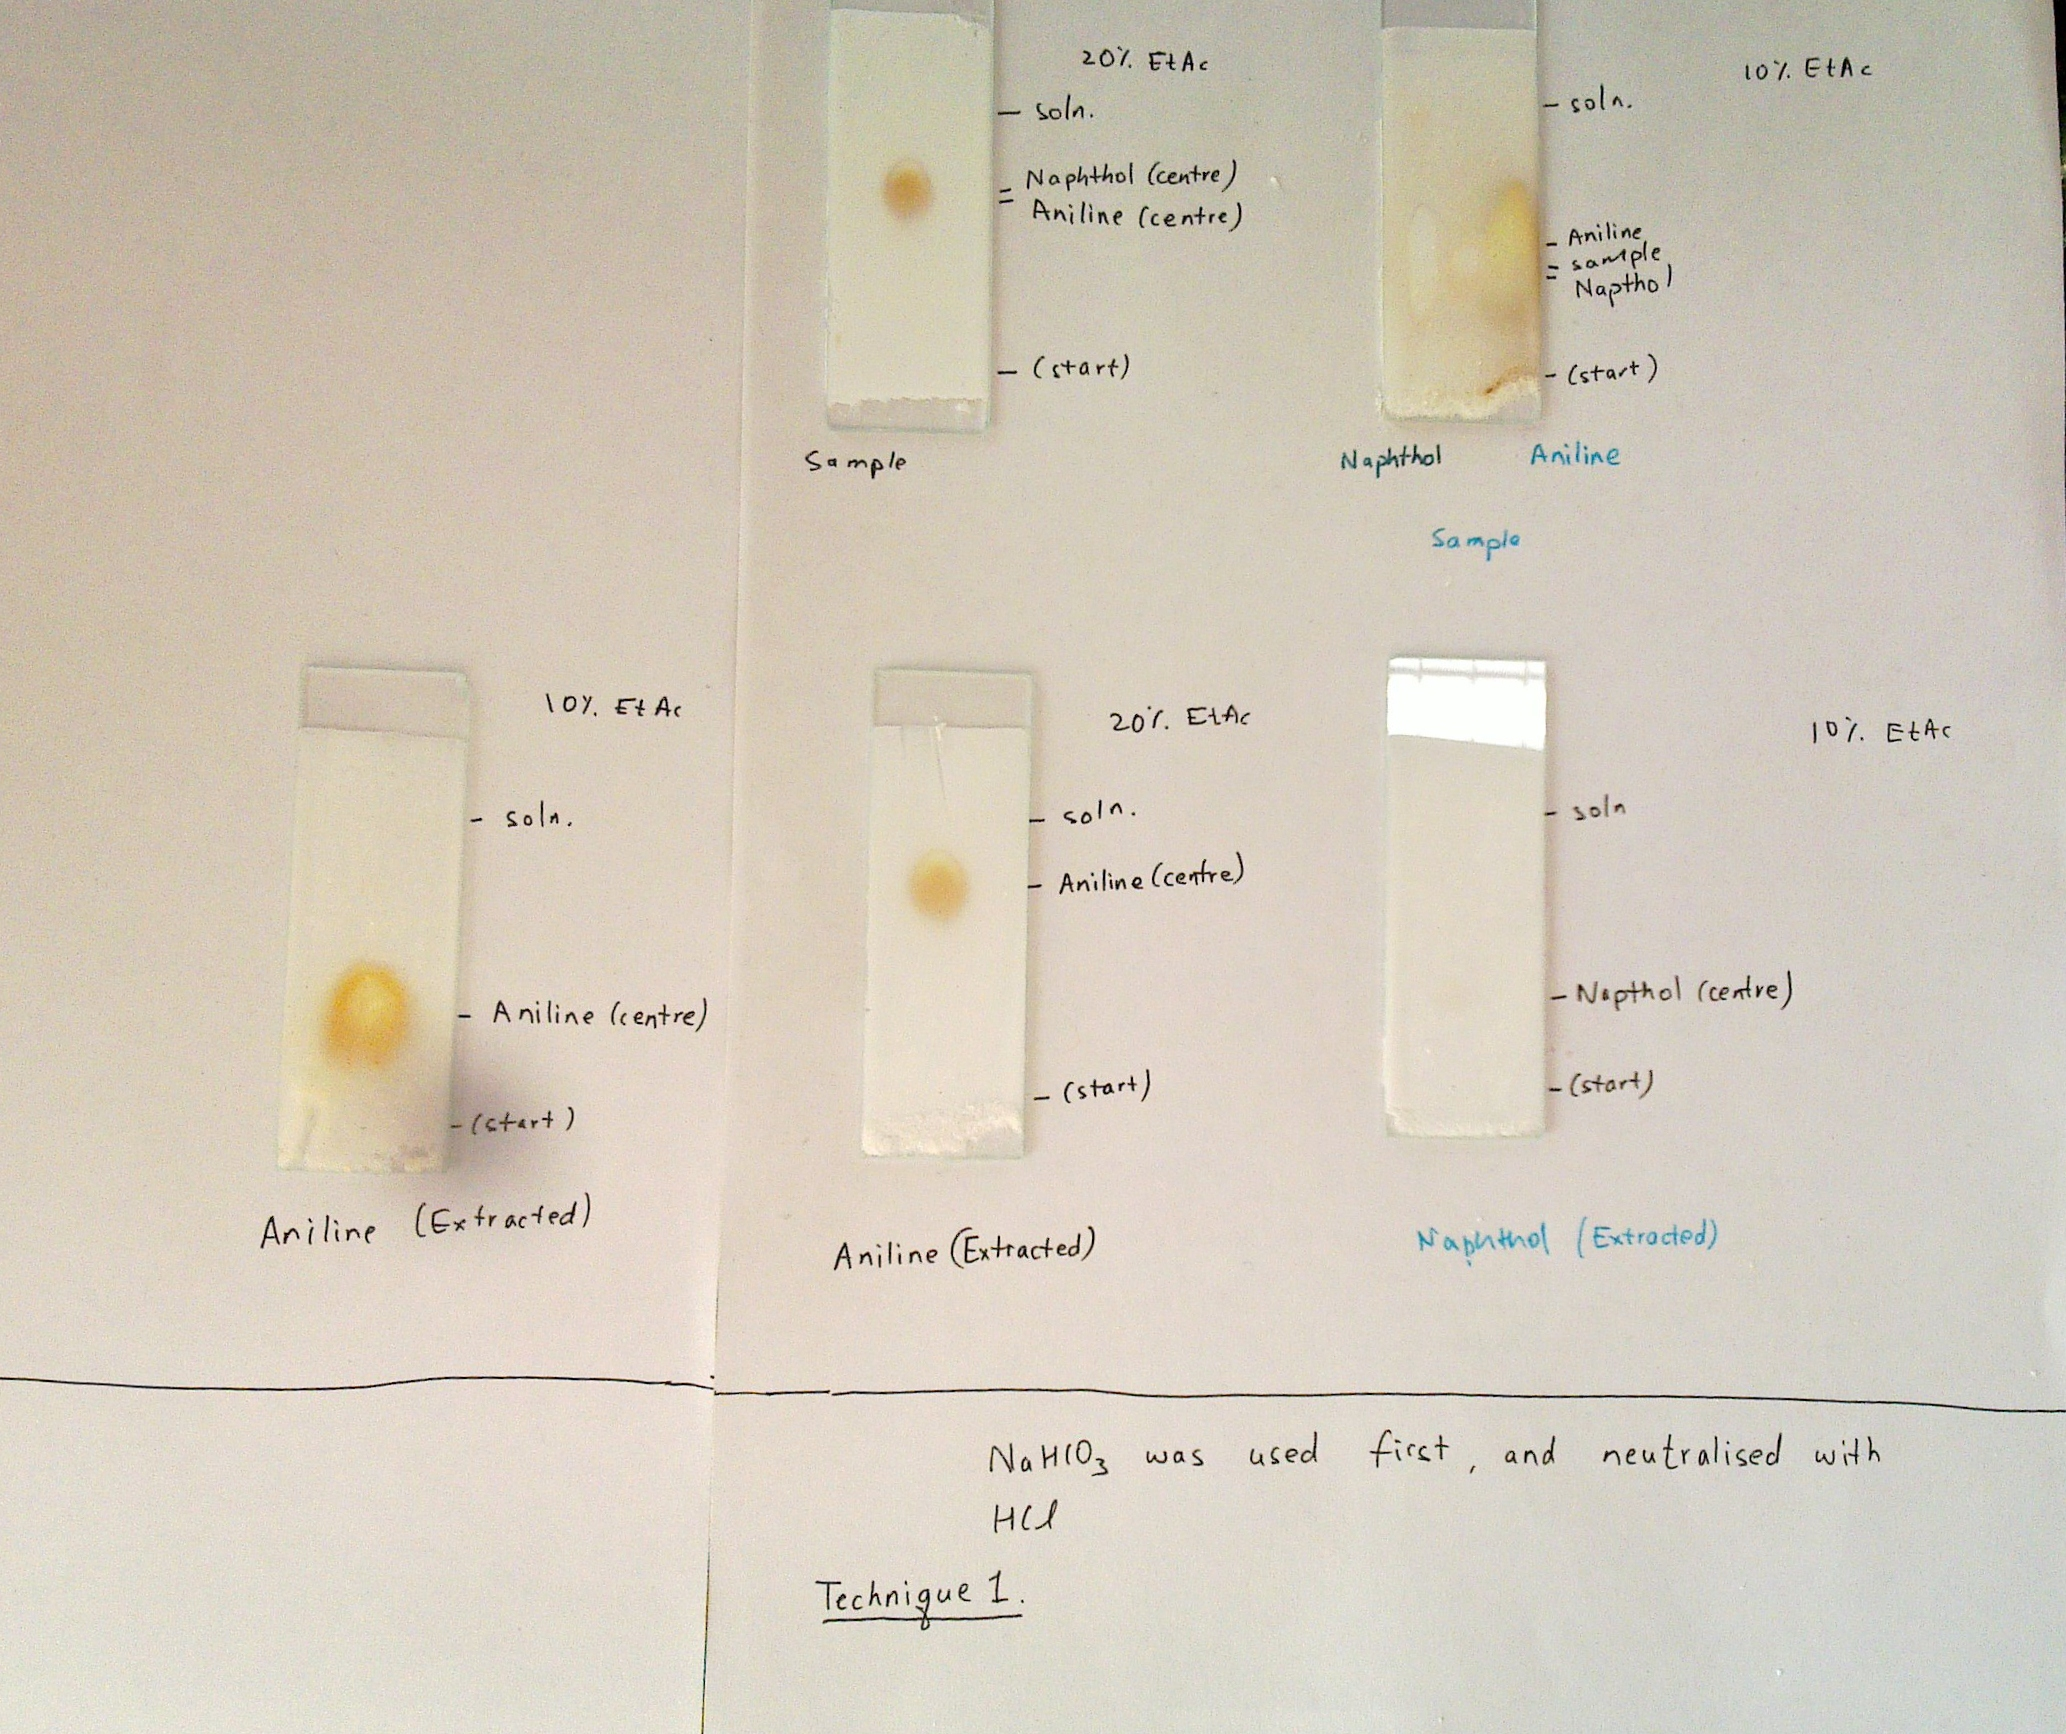
\includegraphics[width=1.5\linewidth]{gfx/e5_1}
		\end{center}
	\caption[TLCs Set 1]{\label{e5_1}}
	\end{figure}

	\begin{figure}[bth]
		\begin{center}
			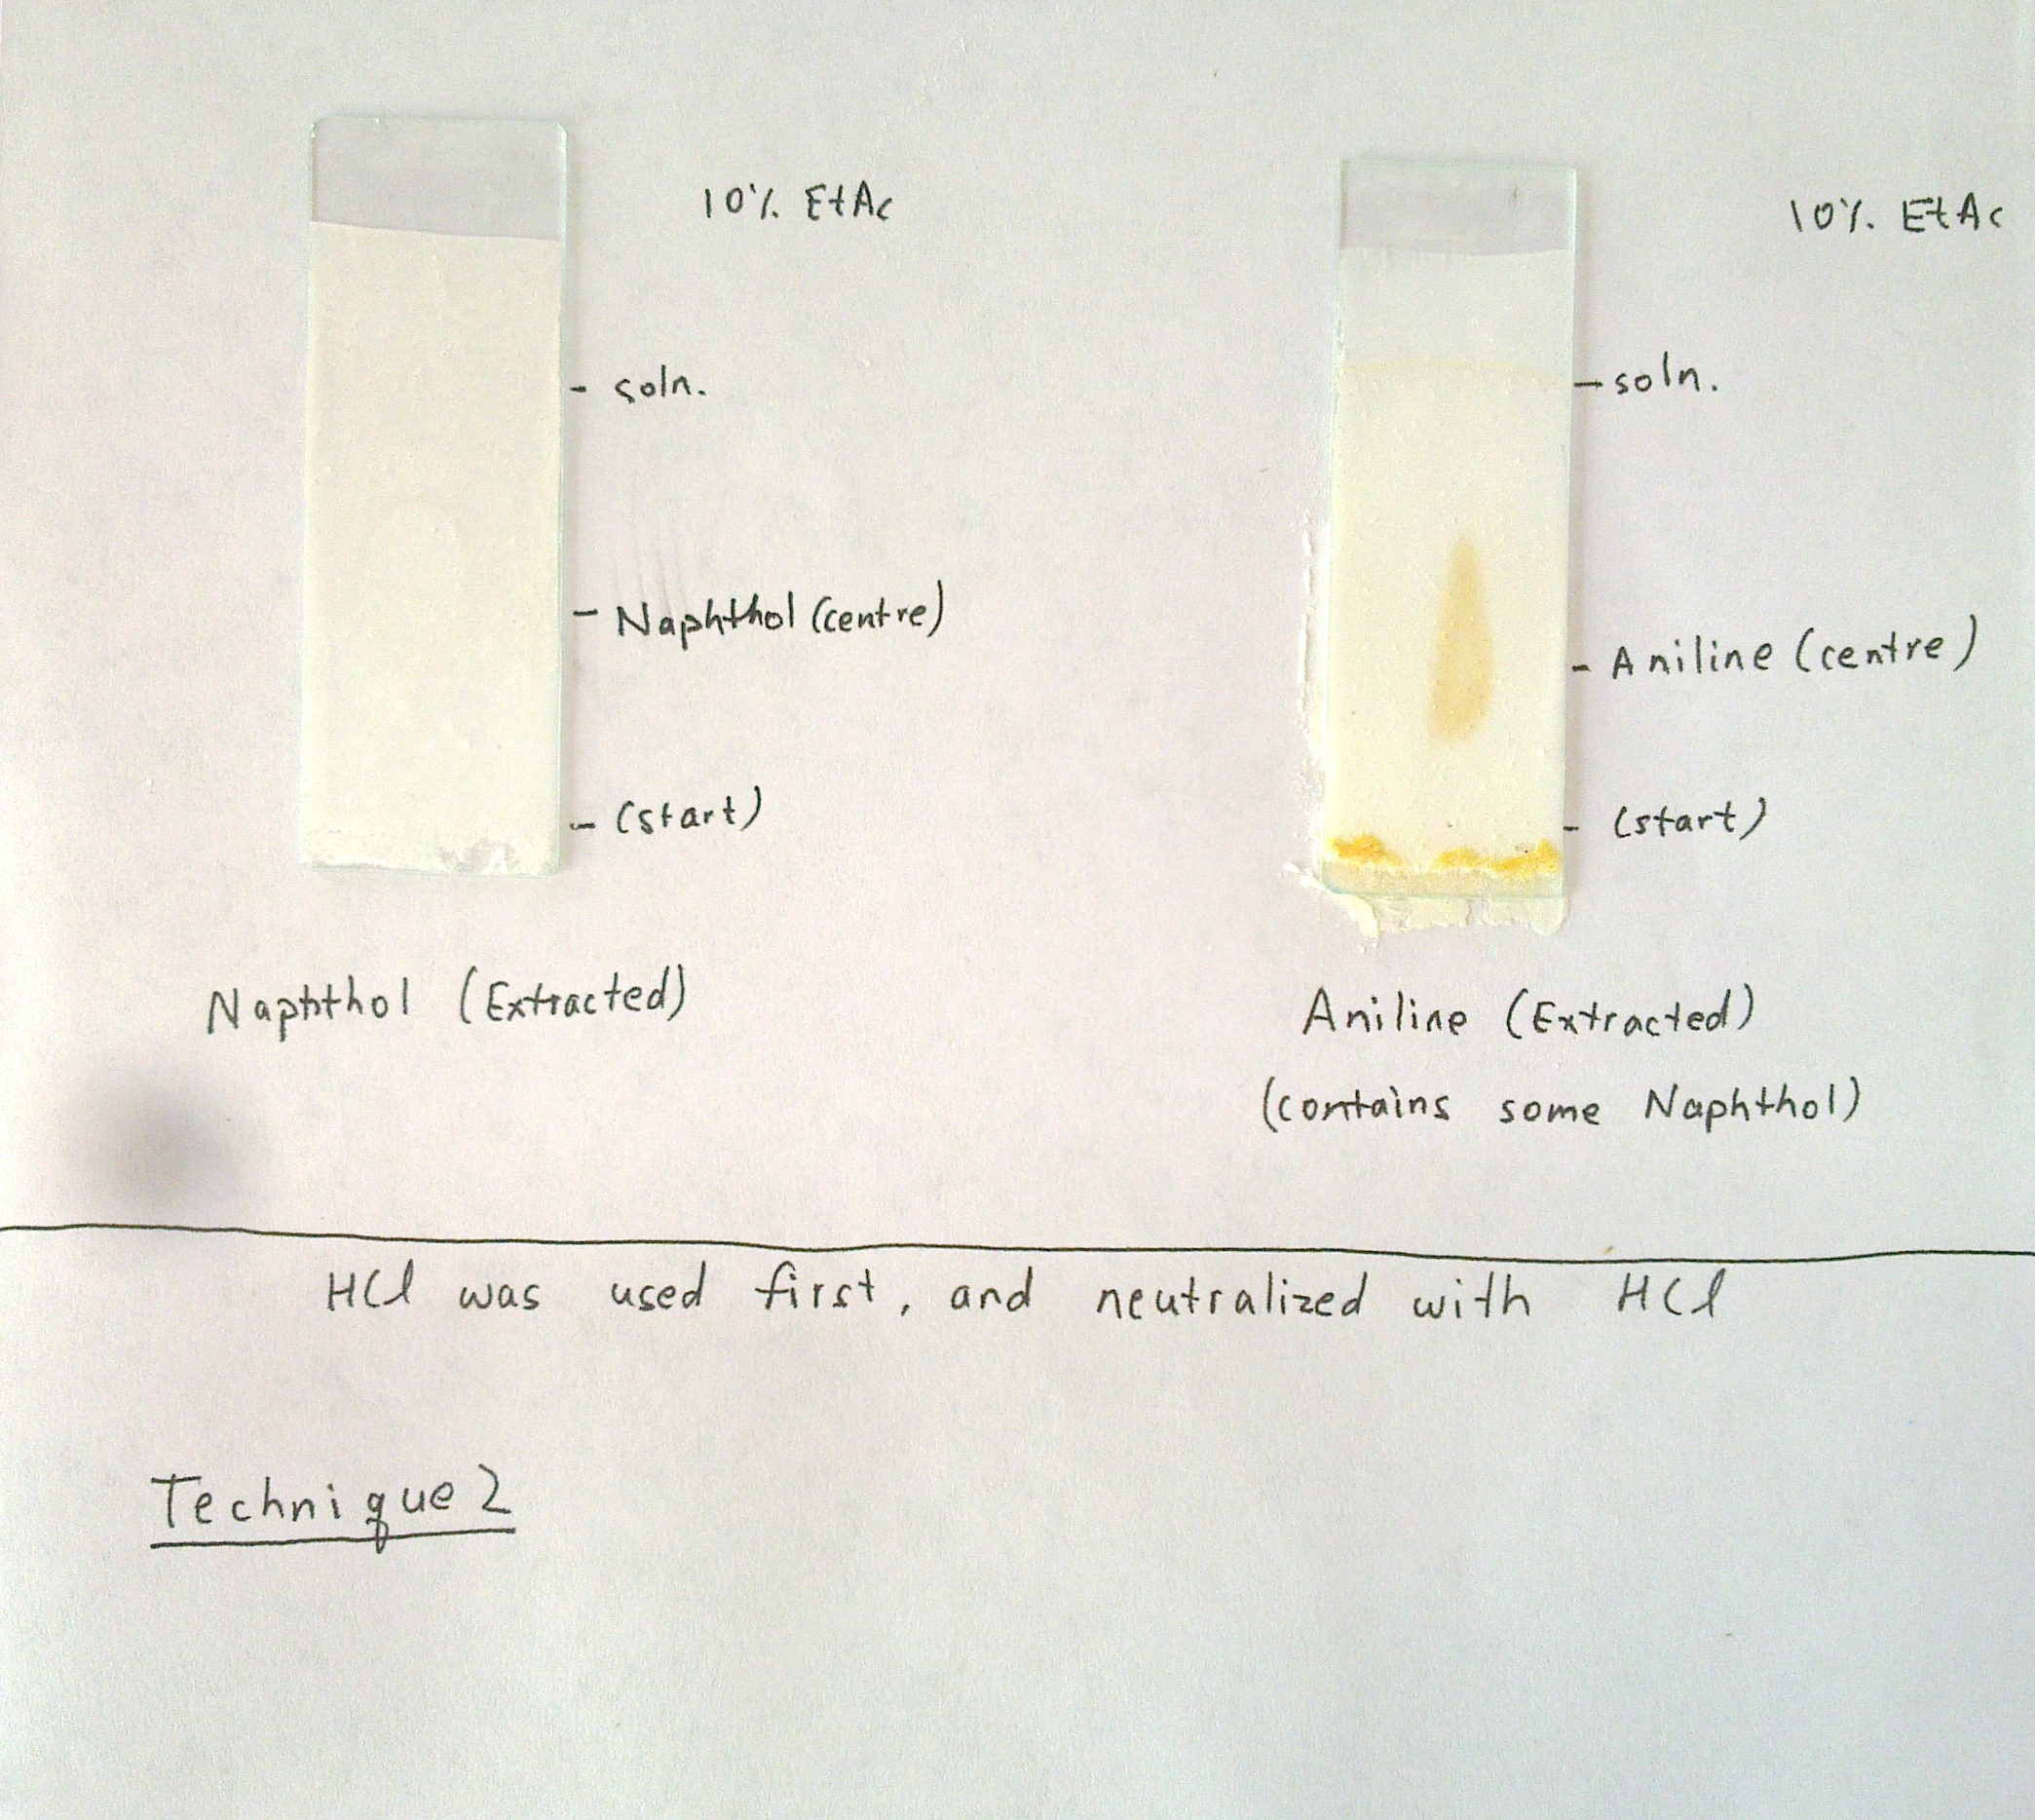
\includegraphics[width=1.0\linewidth]{gfx/e5_2}
		\end{center}
	\caption[TLCs Set 2]{\label{e5_2}}
	\end{figure}